\documentclass[a4paper,11pt,titlepage,dvipdfmx]{jsarticle}


% 数式
\usepackage{amsmath,amsfonts}
\usepackage{bm}

% 画像
\usepackage[dvipdfmx]{graphicx}

% 図形
\usepackage{tikz}
\usetikzlibrary{shapes.geometric}
\usetikzlibrary {shapes.misc}

% ソースコード
\usepackage{listings,jlisting,color}
\lstset{
basicstyle={\ttfamily},
identifierstyle={\small},
commentstyle={\smallitshape},
keywordstyle={\small\bfseries},
ndkeywordstyle={\small},
stringstyle={\small\ttfamily},
frame={tb},
breaklines=true,
columns=[l]{fullflexible},
numbers=left,
xrightmargin=0zw,
xleftmargin=3zw,
numberstyle={\scriptsize},
stepnumber=1,
numbersep=1zw,
lineskip=-0.5ex
}
\renewcommand{\lstlistingname}{ソースコード}


\begin{document}
\begin{titlepage}
    \noindent 
    \vspace{6cm}
    \begin{center}
    \begin{LARGE}
    通信システム実験 第2週 実験レポート
    \end{LARGE}
    \end{center}
    \vspace{6cm}
    \begin{flushright}
    信州大学工学部\\
    電子情報システム工学科\\
    \begin{description}
        \setlength{\leftskip}{8.9cm}
        \item[  実験日:] 2023/04/27 
        \item[ 実験場所:] W2棟601教室
        \item[   気温:] ℃
        \item[   湿度:] \%
        \item[  実験者:] 21T2166D 渡辺 大樹
        \item[共同実験者:] 21T2164H 六川 沙絢
        \item[      ] 21T2167B 渡邉 大翔
        \item[      ] 21T2804J 伊藤 星斗
    \end{description} 
    \end{flushright}
\end{titlepage}


\section{目的と概要}
本実験ではArduinoを用いてマイコンの制御、また前回用いたソフトであるIFTTTを用いて近年話題となっているIoT(Internet of Things)についての理解を用いる。

\subsection{事前学習}
本実験の事前学習として以下Arduinoの標準ライブラリ、
もしくは実験にて使用する温湿度センサー(DHT11)を用いるために用意されているライブラリのDHT.h
にある7つの主な関数について調べた。上記4つの関数はArduino公式リファレンスの有志の日本語訳サイト\cite{ref}を参考にしている。
DHTライブラリの関数は公式ドキュメントが見つからなかったため、配布元のGitHub\cite{DHTgit}にあったテストコードのコメントを参考に作成している。
以下がその関数と調べた結果になる。
\begin{description}
    \item[・Serial.print()]\mbox{}\\
    この関数は引数に来た文字、数字をシリアルポートにASCIIテキストとして出力する。
    浮動小数点はデフォルトだと小数点以下第2位までが送信される。これは第2引数で変更することができる。
    \item[・digitalRead(pin)]\mbox{}\\
    この関数は引数にデジタルピンの番号を取り、引数に指定したピンからHIGHもしくはLOWの値を読み取り、返す。
    \item[・digitalWrite(pin, value)]\mbox{}\\
    この関数は第1引数にデジタルピンの番号、第2引数にHIGHもしくはLOWを取る。
    この引数に、OUTPUTに設定されているピンを指定したときはピンの電圧がvalueに沿ってHIGH(3.3V)もしくはLOW(0V)になる。
    逆にINPUTに設定されたピンを入力したときは、ピン内部のプルアップ抵抗の有効無効を切り替えることでができる。
    \item[・pinMode(pin, mode)]\mbox{}\\
    この関数は第1引数で指定したピンを第2引数で入力に使うのか出力に使うのかを設定する。
    第2引数のModeにはINPUTもしくはOUTPUT、またINPUT PULLUPが入る。
    ModeをINPUT PULLUPにすることで内部のプルアップ抵抗を有効にすることが可能である。
    \item[・dht.begin()]\mbox{}\\
    この関数はDHTセンサーを初期化するための関数である。
    \item[・dht.readTemperature()]\mbox{}\\
    この関数はDHTセンサーから温度を読み取る関数である。戻り値として温度が出力される。
    引数に何もセットしなかった場合、Celsius温度を、Trueを入力するとFahrenheit温度を出力する。
    \item[・dht.readHumidity()]\mbox{}\\
    この関数はDHTセンサーから湿度を読み取る関数である。戻り値として湿度が出力される。
\end{description}

\section{実験内容}
本実験ではArduinoを用いて二種の実験を行う。

実験1では赤外線モジュールを用いて赤外線通信を受信する実験を行う。
赤外線モジュールとArduinoと接続し、eAlps記載のコードをコンパイル、書き出して実行する。
実行したのちに実際に赤外線通信を行っているリモコンをモジュールに向けて操作することで赤外線を受信する。

実験2ではArduinoとIFTTTを用いて、温湿度センサーからArduinoで取得した温度をWeb上で確認する実験を行う。
温湿度センサーにはDHT11を用いてArduinoと接続し、eAlps記載のコードをコンパイル、書き出して実行する。
コードではArduinoを601教室のネットワークに接続し、ArduinoからIFTTTにWebリクエストを行って、
URLパラメータを用いて温湿度センサーから得た温度をIFTTTに送信している。
\section{結果}
以下に実験の結果を記す。
\subsection{実験1}
実験1では以下図1のような回路を実装し、実験した。
\begin{figure}[h]
    \begin{center}
        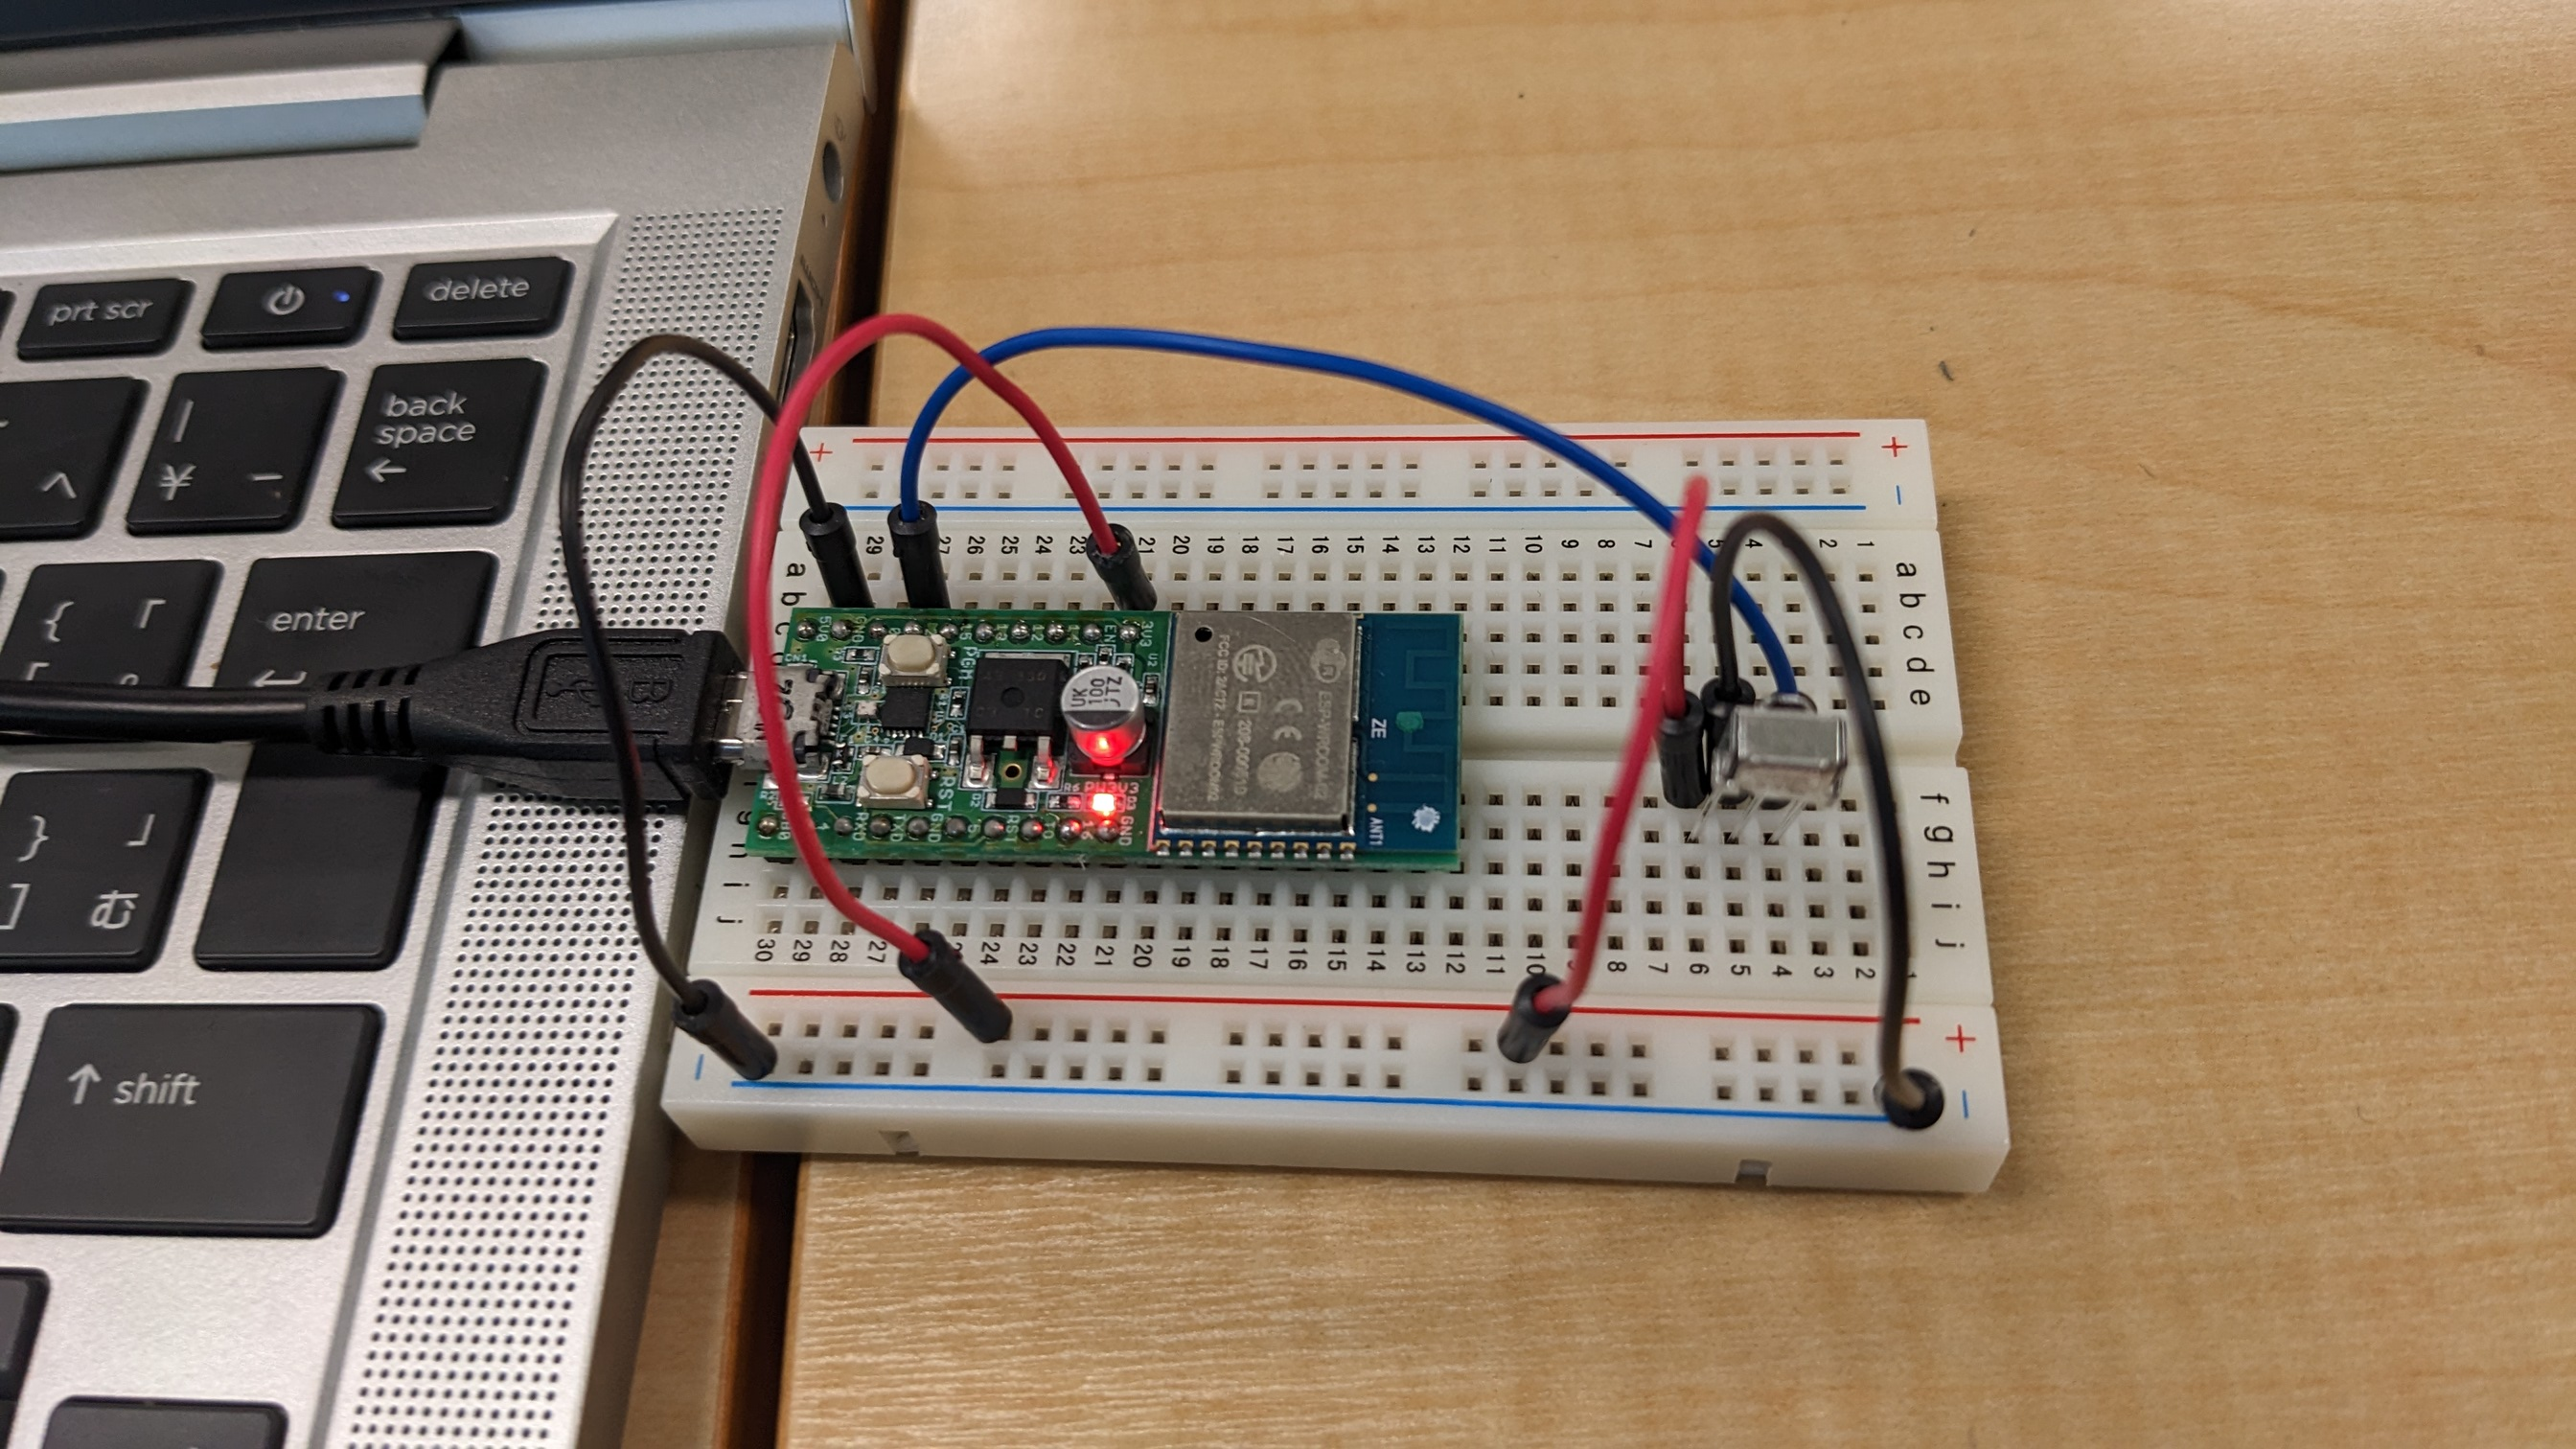
\includegraphics[width=100mm]{./circuit.jpg}
    \end{center}
    \caption{実験1で実装した回路}
\end{figure}

またこの図1の回路にリモコンで赤外線を当てたところ、以下図2のような出力が得られた。
\begin{figure}[h]
    \begin{center}
        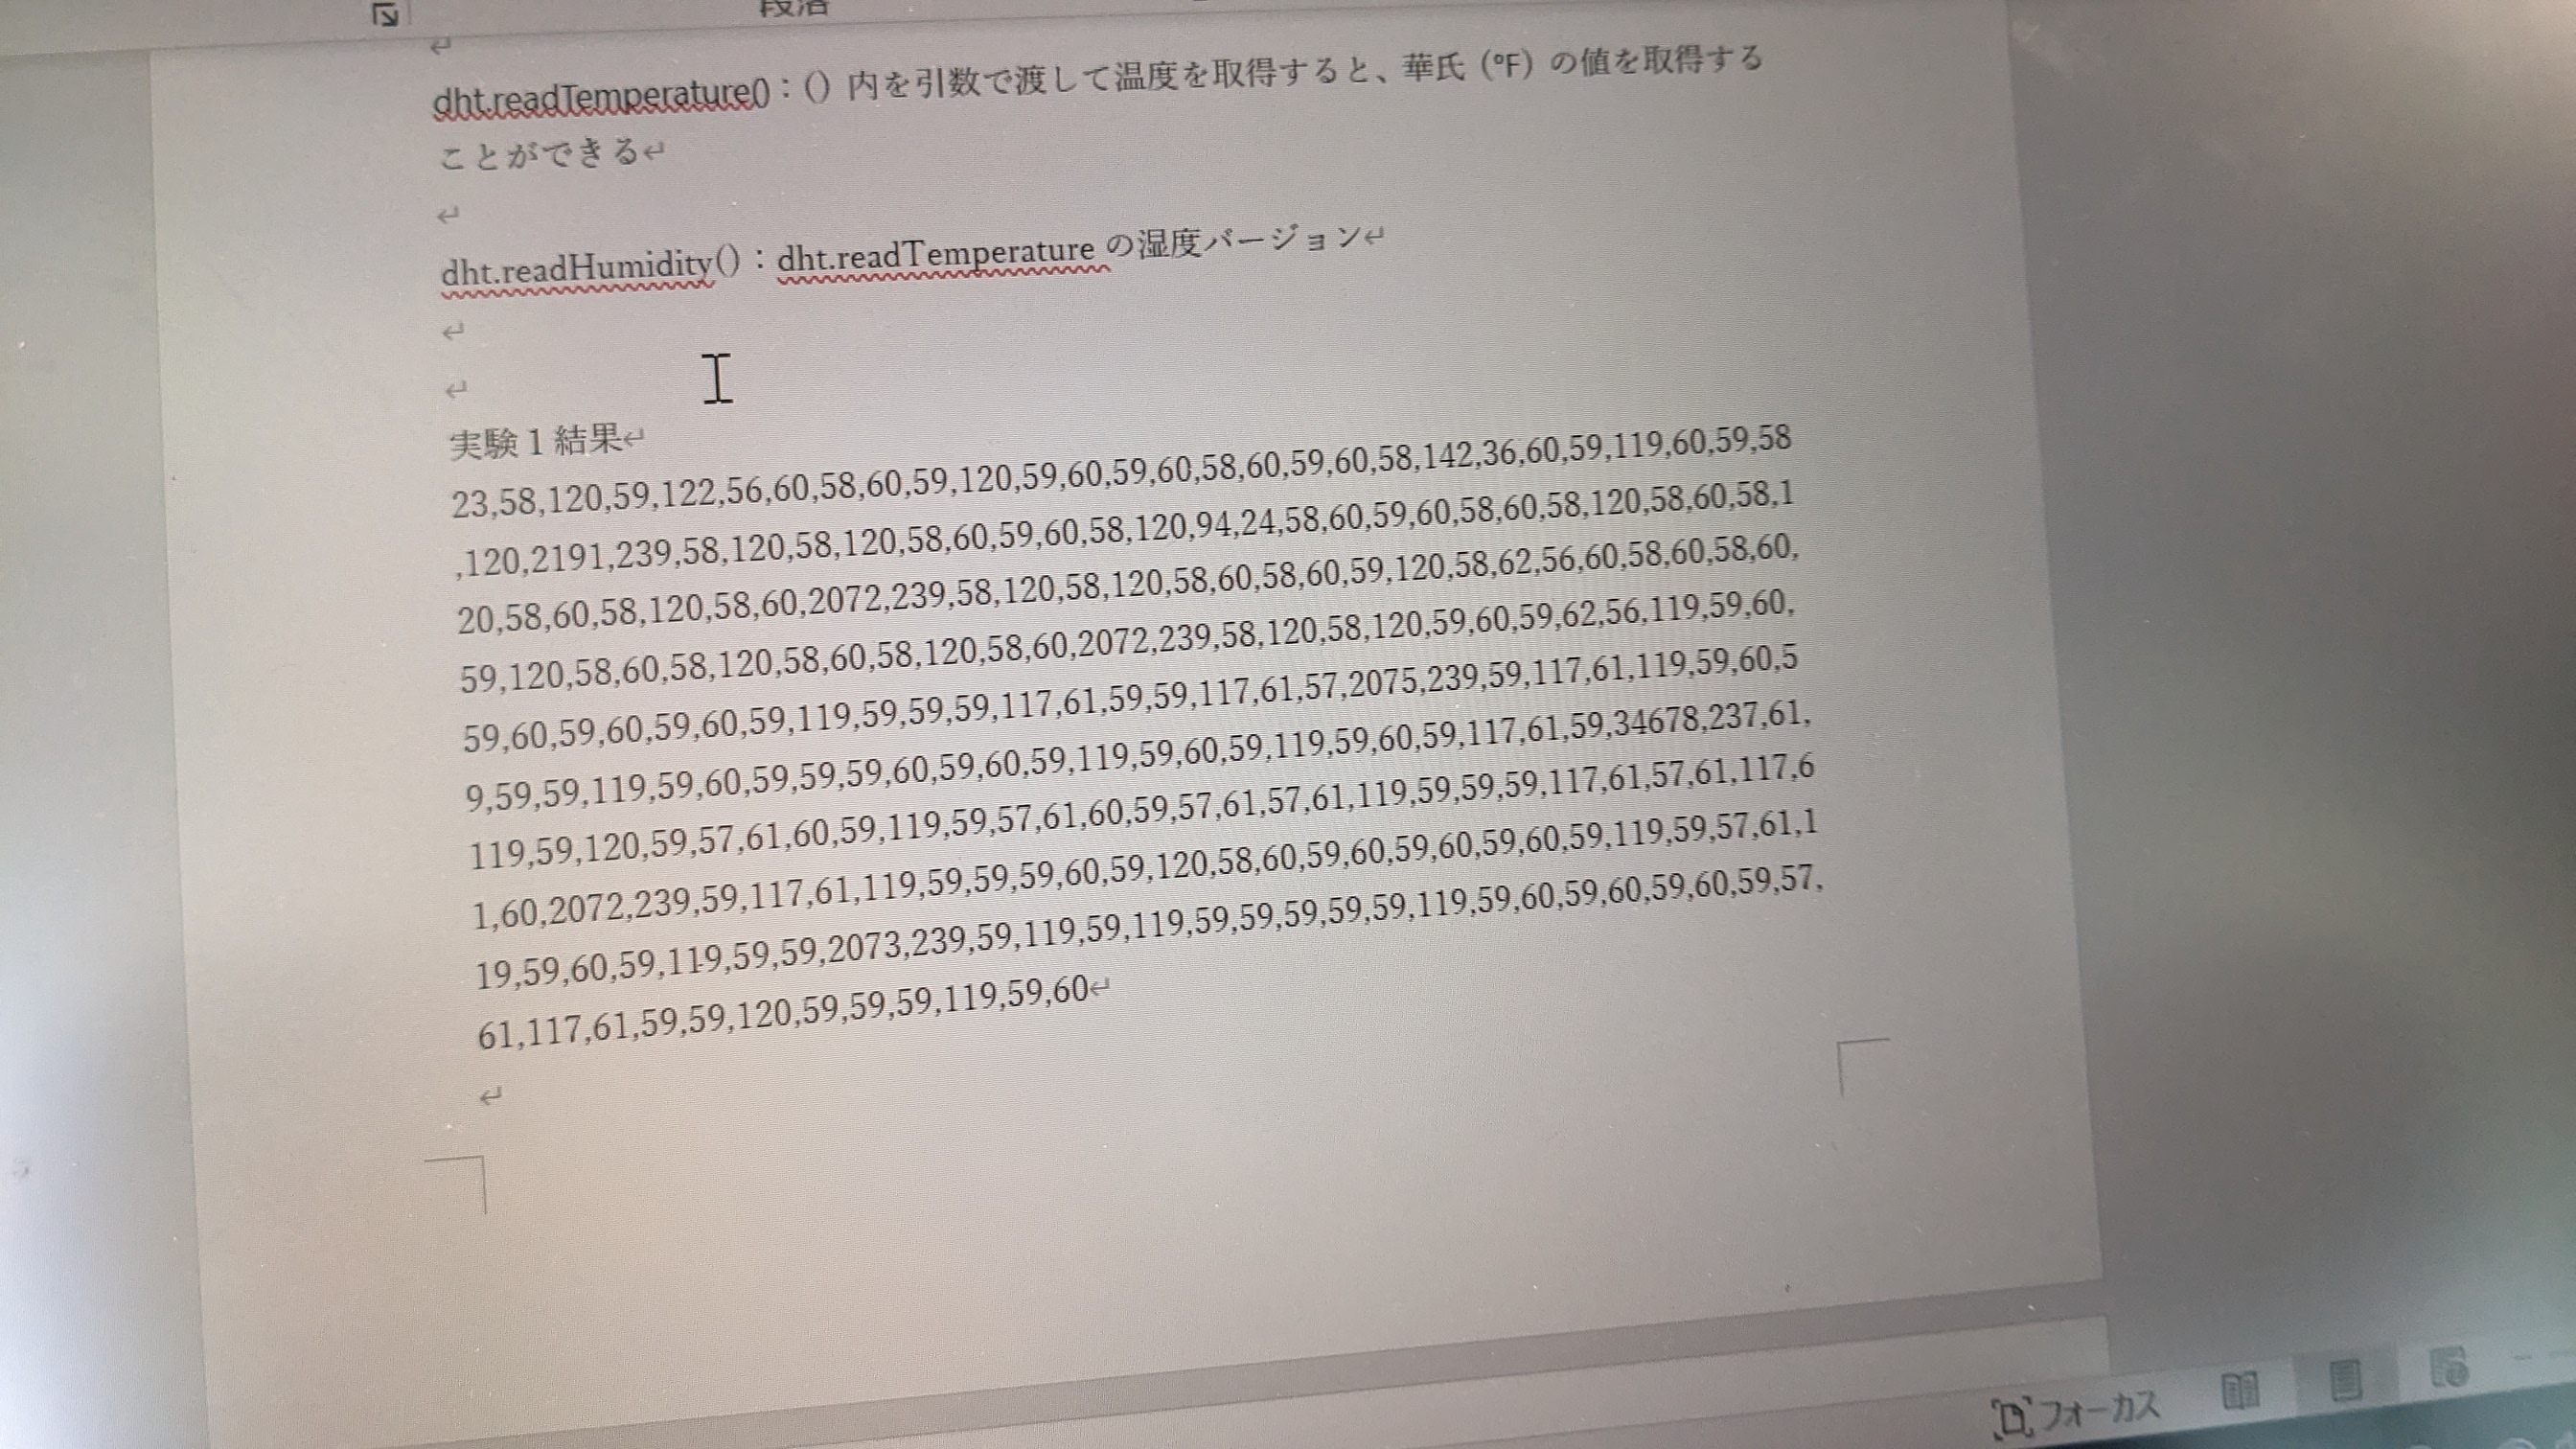
\includegraphics[width=100mm]{./infredrays.jpg}
    \end{center}
    \caption{実験1での出力}
\end{figure}
\newpage

\subsection{実験2}
実験2では以下図3のような回路を実装し、実験した。
\begin{figure}[h]
    \begin{center}
        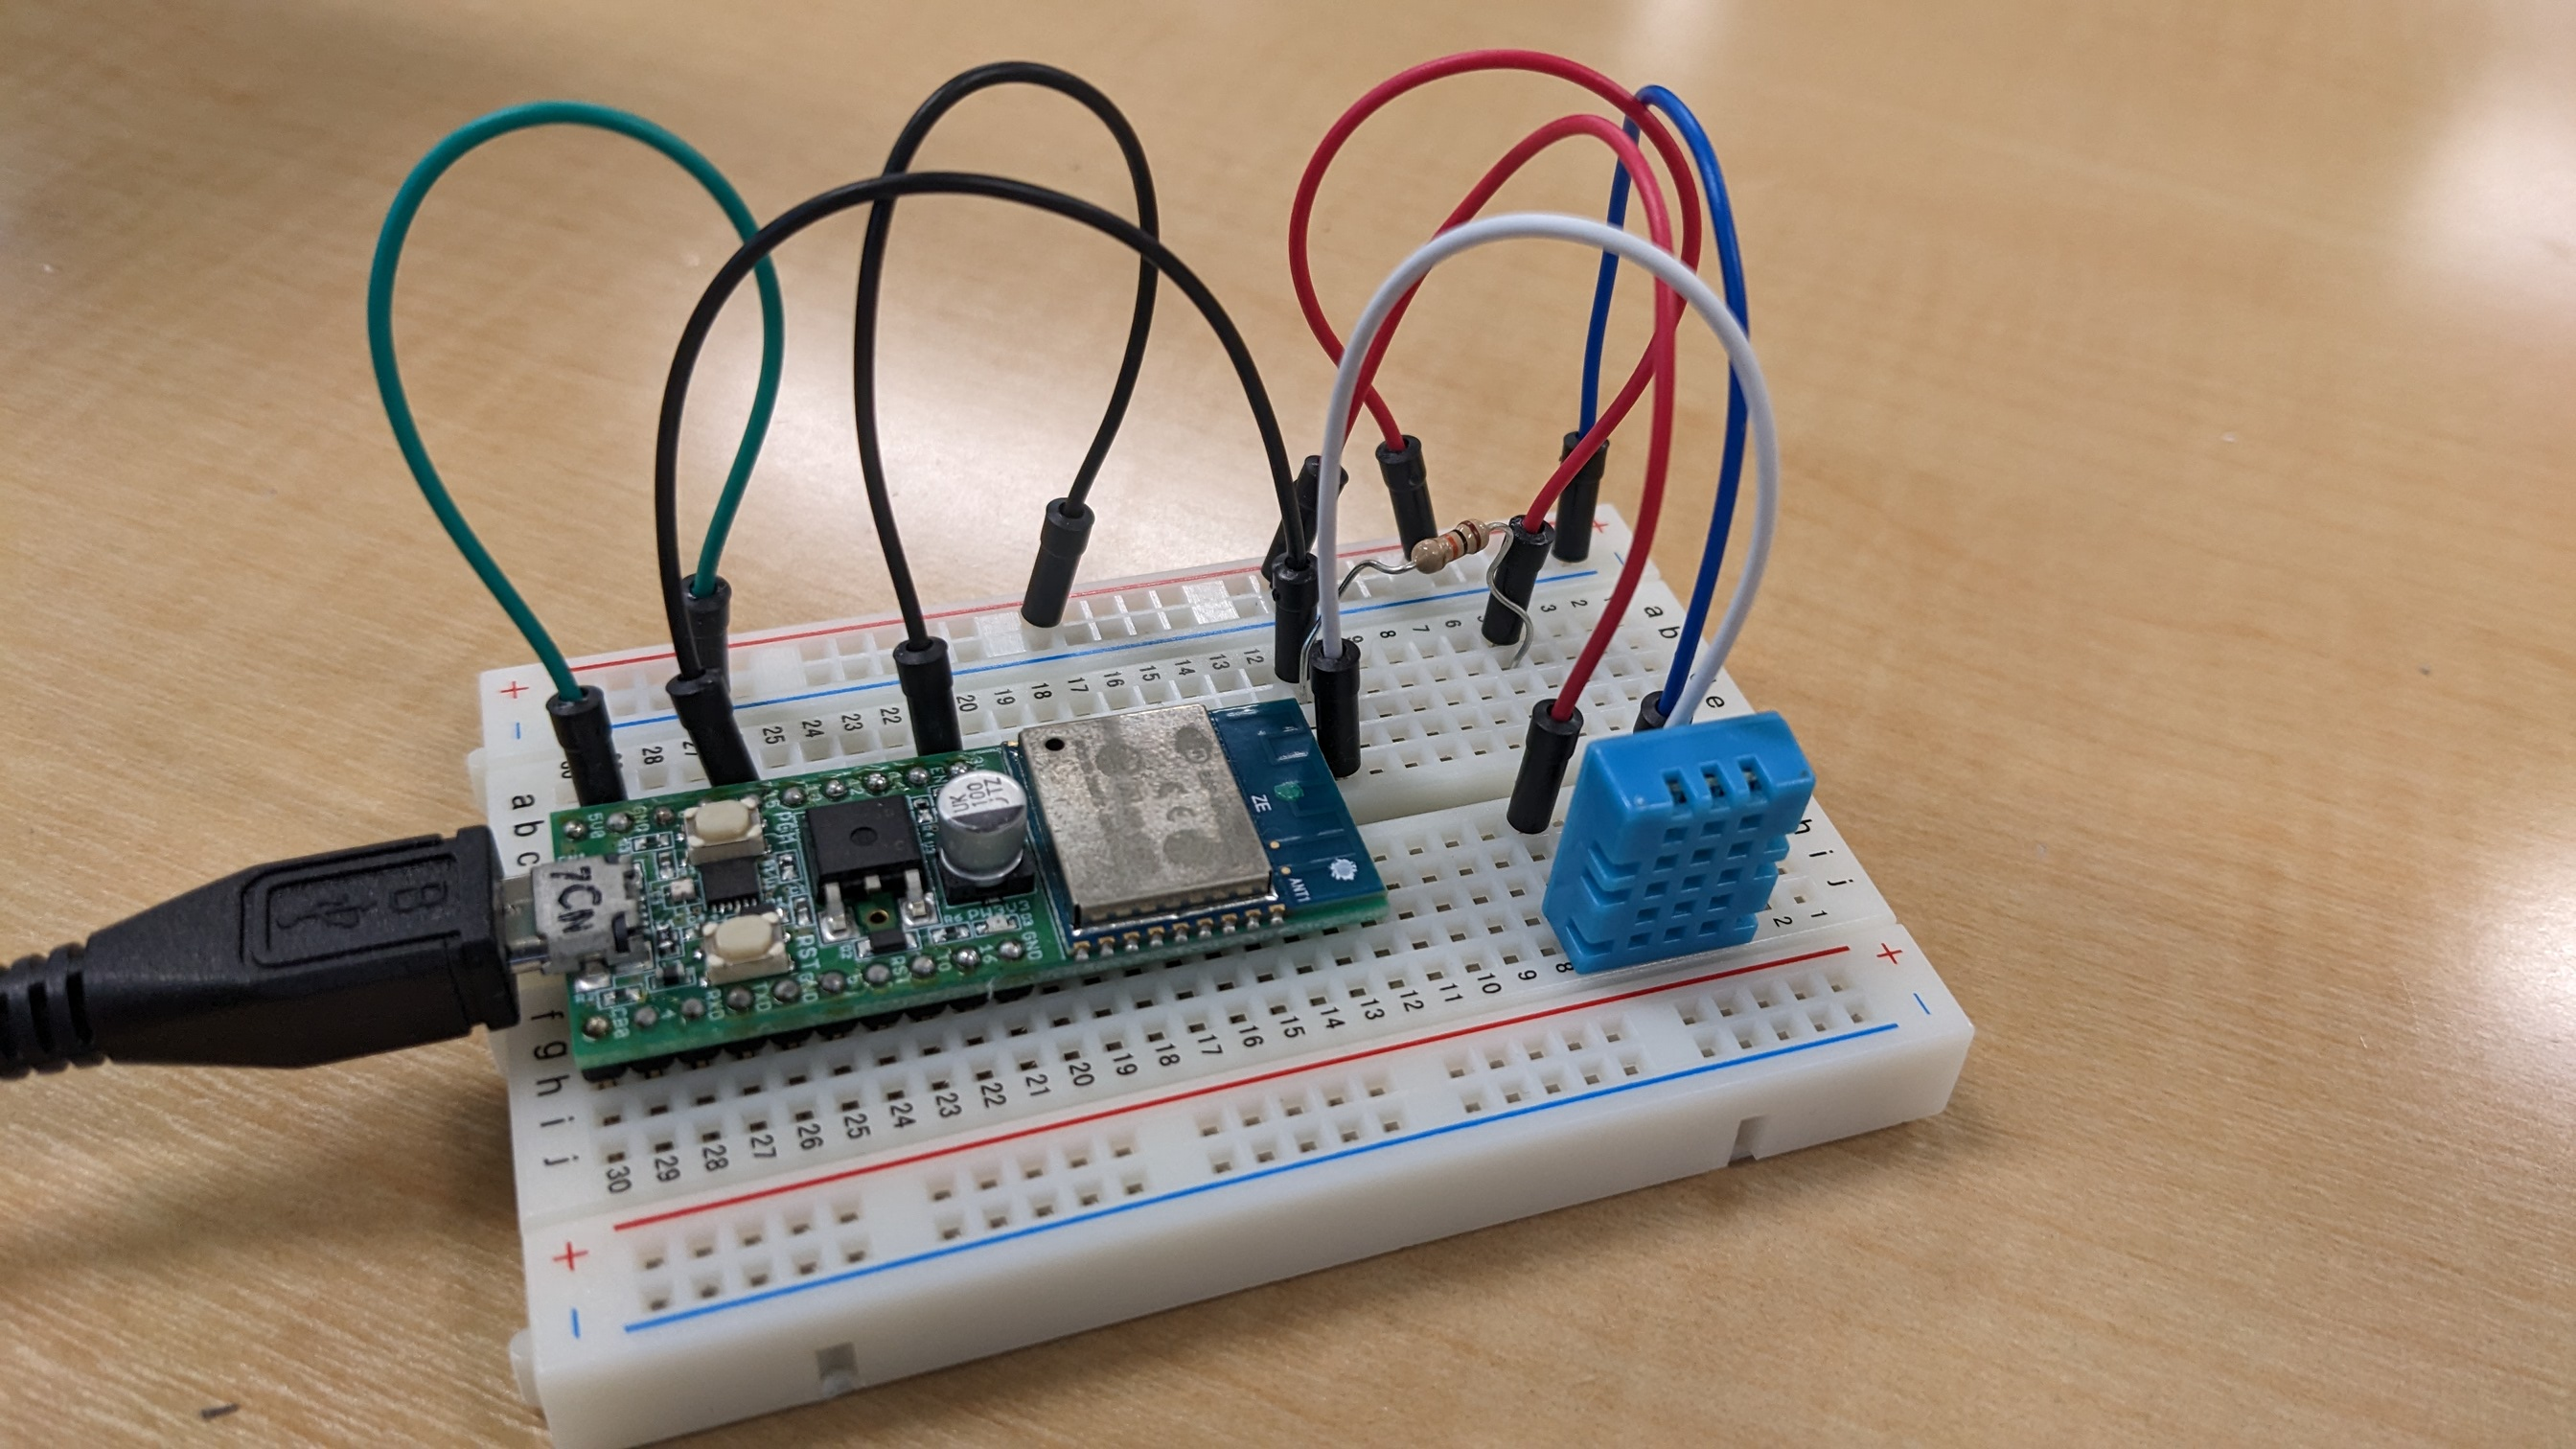
\includegraphics[width=100mm]{./circuit2.jpg}
    \end{center}
    \caption{実験2で実装した回路}
\end{figure}

またこの図3の回路を動作させ、IFTTTにアクセスしたところ以下図4のような結果を得られた。
\begin{figure}[h]
    \begin{center}
        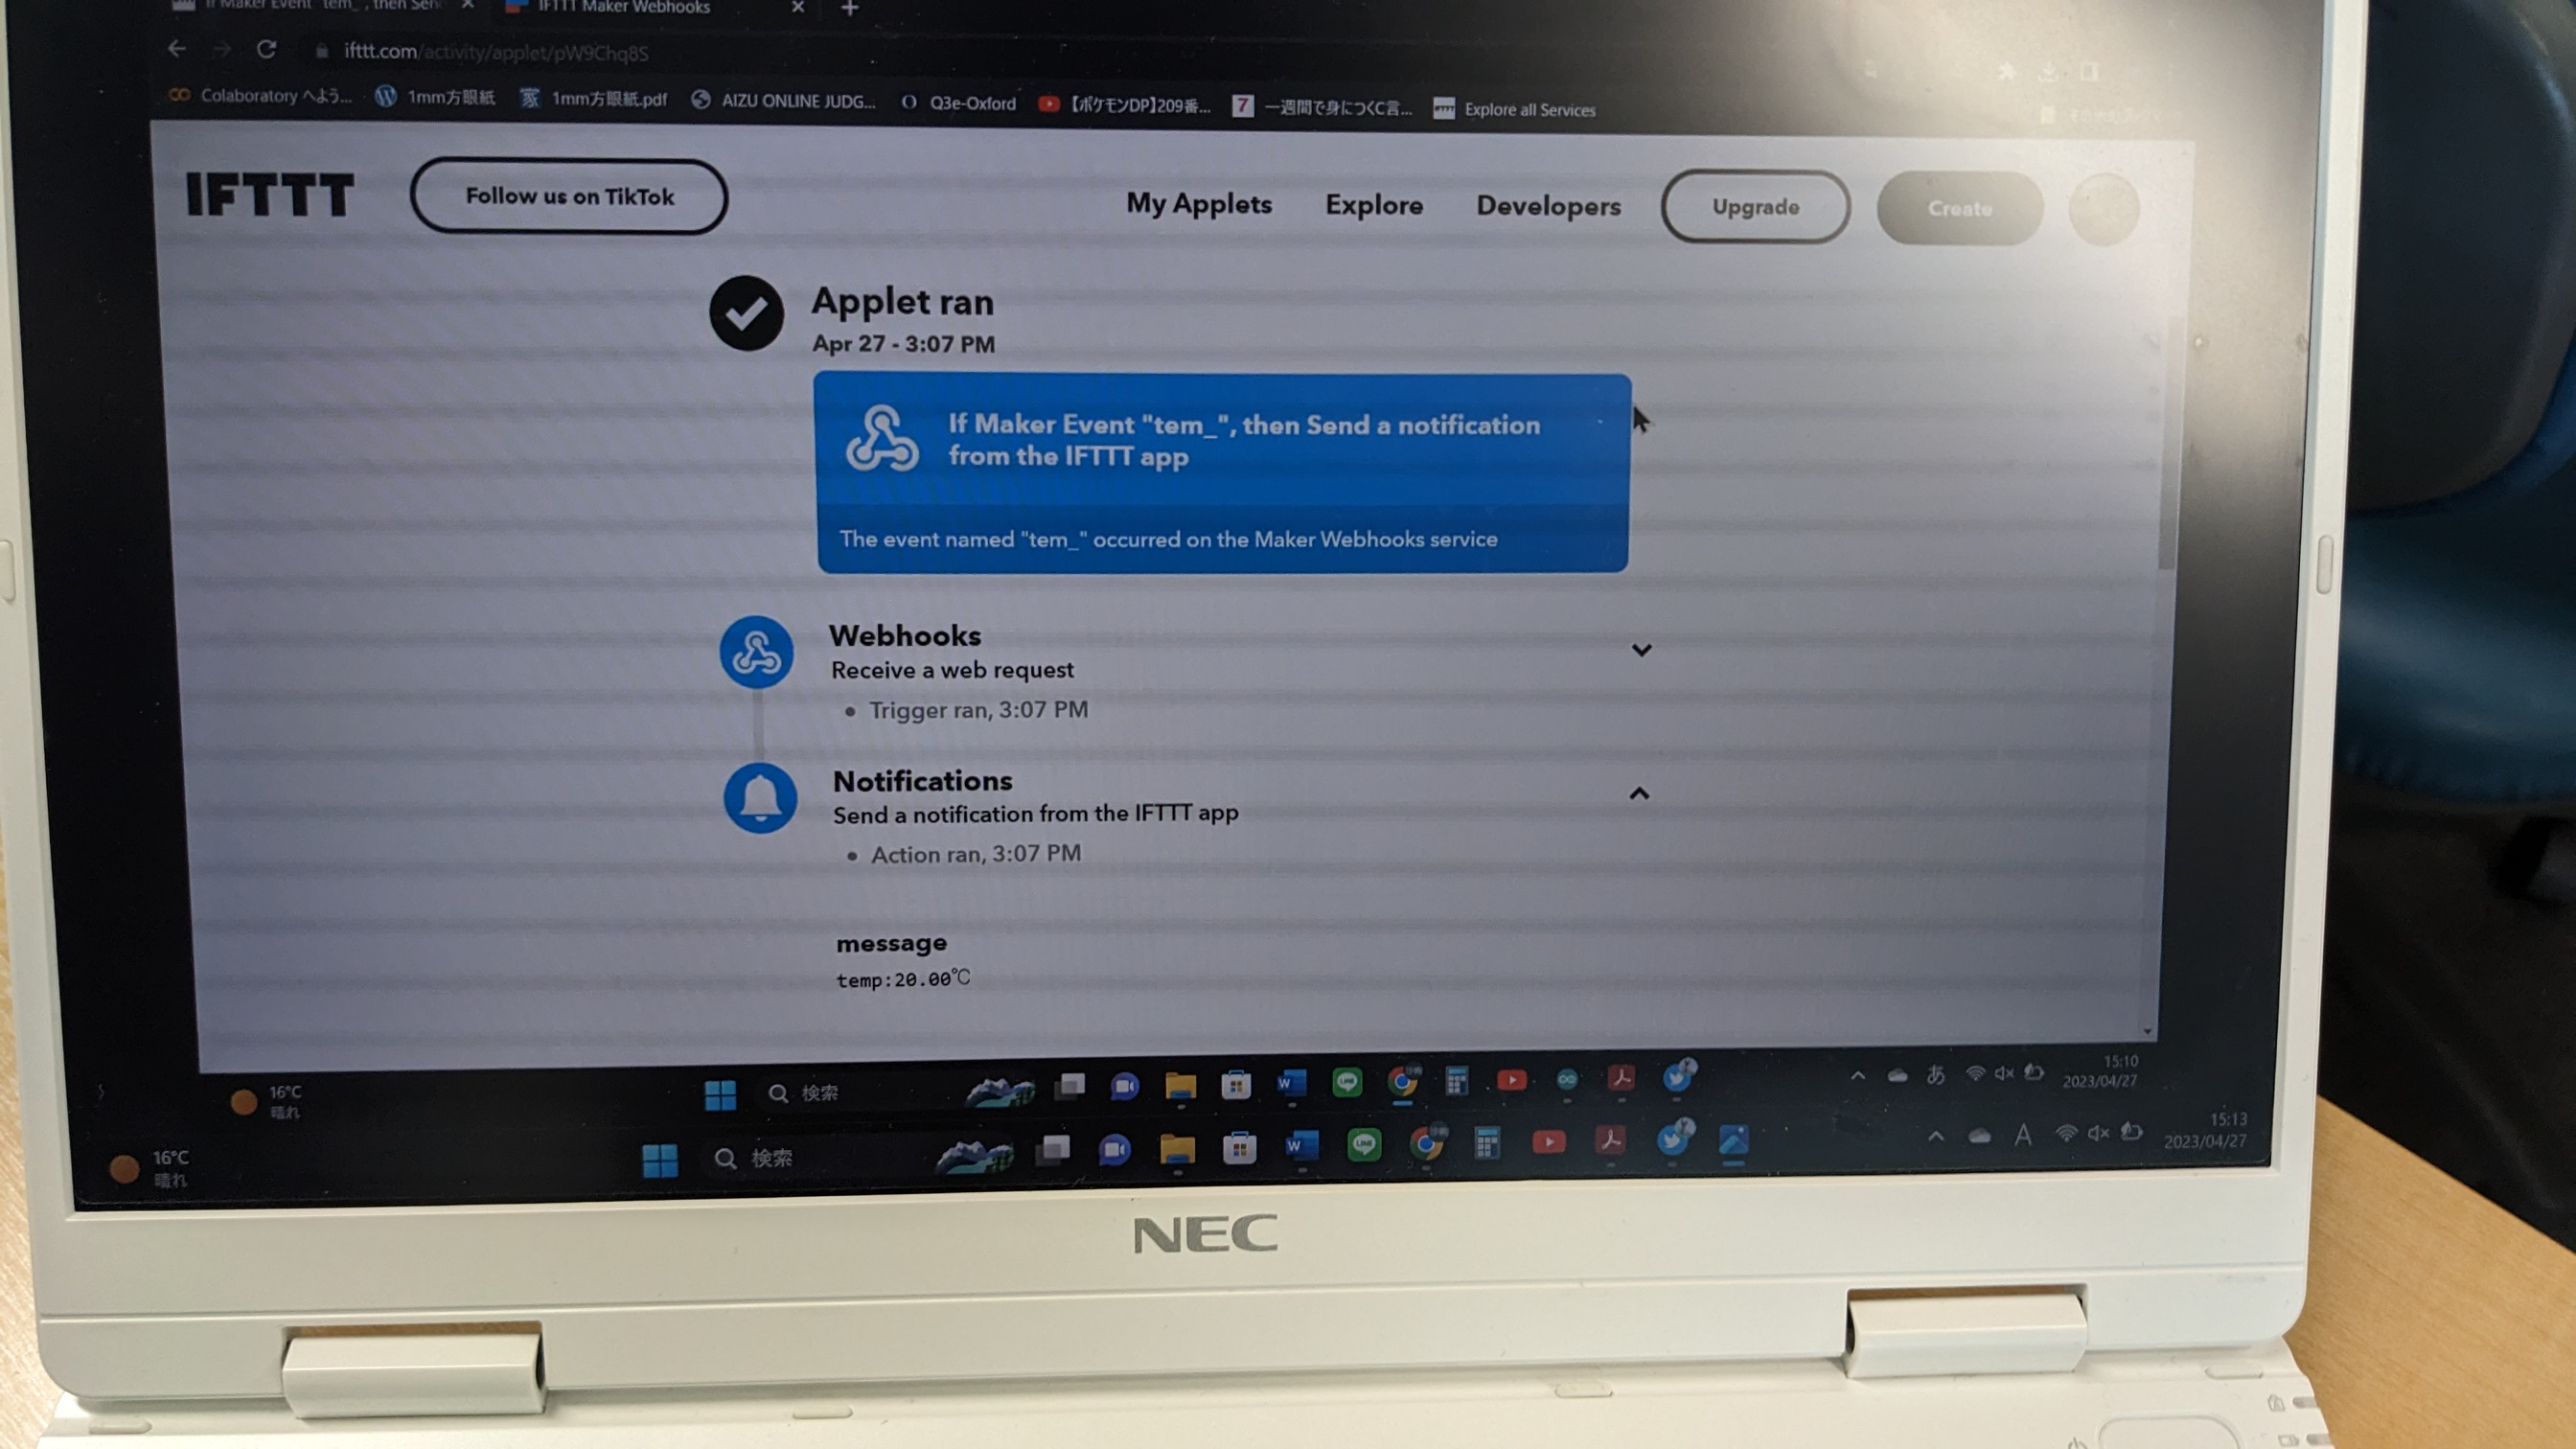
\includegraphics[width=100mm]{./Temp.jpg}
    \end{center}
    \caption{実験2でのIFTTTの出力}
\end{figure}
\newpage

\section{考察}
以下にこの実験での考察を示す。
\subsection{実験1}
実験1の結果、特に図2の結果から考察していく。図2ではリモコンからの赤外線の状態が変わらなかった時間が出力されており、
このデータだけでは分析しずらいもののある程度周期的に変化しているのが分かる。特に59、119近傍の数字がよく出力されていることを
考えると実験で用いたリモコンは590$\mu s$ごとに振幅の変わる信号を用いているのではと推測した(つまり振幅変調?)。

また資料に記載されていたプログラム全文を載せることはできないため、以下に実験1で用いたコードのフローチャートを作成した。
このフローチャートは \LaTeX のTi\emph{k}Zを用いて作成しているが、不慣れのためloopの処理は台形での表示としている。

\newpage
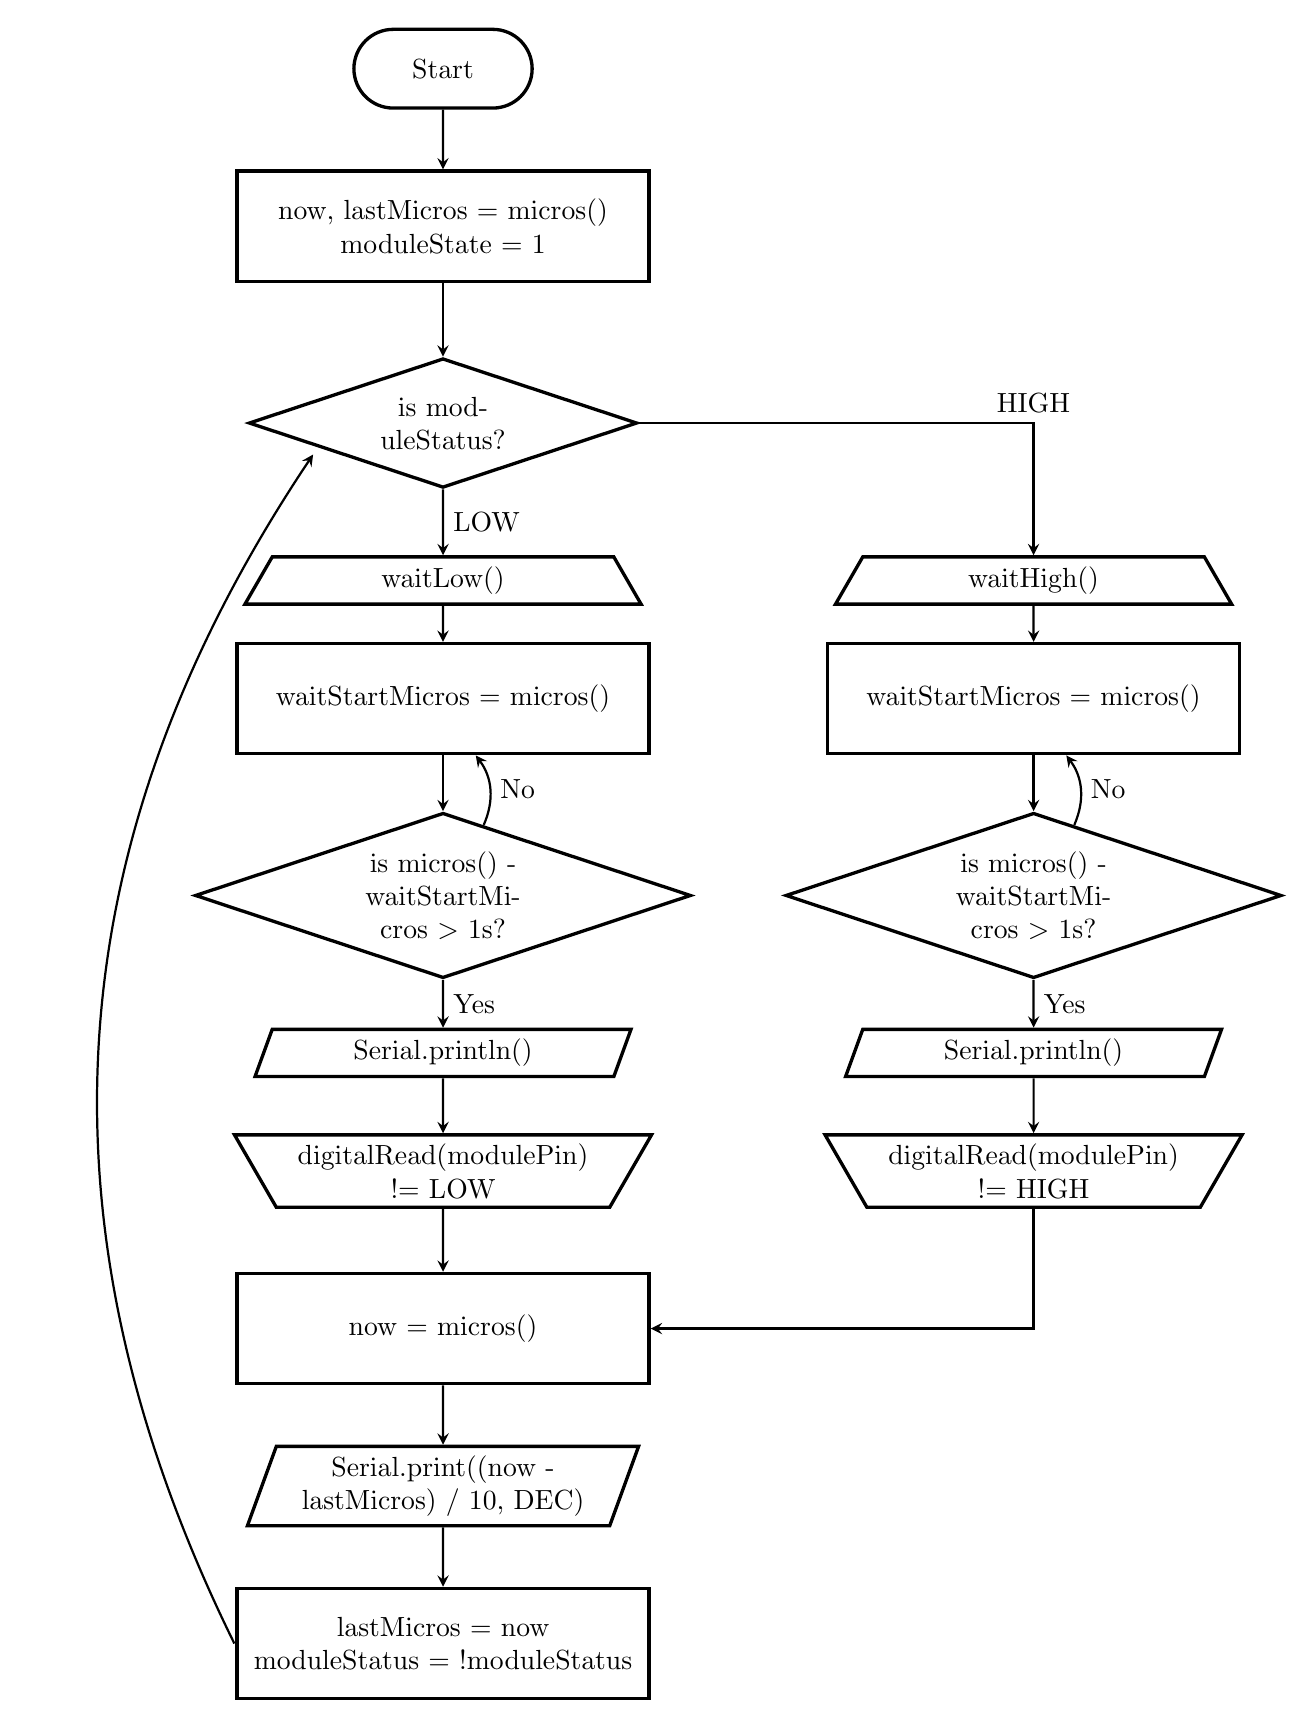
\begin{tikzpicture}[very thick]
\tikzset{Terminal/.style={rounded rectangle,  draw,  text centered, text width=2cm, minimum height=1cm}};
\tikzset{Process/.style={rectangle,  draw,  text centered, text width=5cm, minimum height=1.4cm}};
\tikzset{ifthen/.style={diamond,  draw,  text centered, aspect=3,text width=2cm, minimum height=1cm}};
\tikzset{InOut/.style={trapezium, draw, text centered, text width=4cm, minimum height=0.6cm, trapezium left angle=70, trapezium right angle=110}};
\tikzset{LoopStart/.style={trapezium, draw, text centered, text width=4cm, minimum height=0.6cm, trapezium angle=60}};
\tikzset{LoopStop/.style={trapezium, draw, text centered, text width=4cm, minimum height=0.6cm, trapezium angle=120}};
\tikzset{arrow/.style={thick, ->, >=stealth}};

\node[Terminal](a)at (0,0){Start};
\node[Process](b)at (0,-2){now, lastMicros = micros()\\moduleState = 1};
\node[ifthen](c)at (0,-4.5){is moduleStatus?};
\node[LoopStart](d1)at (7.5,-6.5){waitHigh()};
\node[Process](d)at (7.5,-8){waitStartMicros = micros()};
\node[LoopStart](e1)at (0,-6.5){waitLow()};
\node[Process](e)at (0,-8){waitStartMicros = micros()};
\node[ifthen](f)at (7.5,-10.5){is micros() - waitStartMicros $>$ 1s?};
\node[ifthen](g)at (0,-10.5){is micros() - waitStartMicros $>$ 1s?};
\node[InOut](h1)at (7.5,-12.5){Serial.println()};
\node[InOut](h2)at (0,-12.5){Serial.println()};
\node[LoopStop](i1)at (7.5,-14){digitalRead(modulePin) != HIGH};
\node[LoopStop](i2)at (0,-14){digitalRead(modulePin) != LOW};
\node[Process](i)at (0,-16){ now = micros()};
\node[InOut](j)at (0,-18){Serial.print((now - lastMicros) / 10, DEC)};
\node[Process](k)at (0, -20){lastMicros = now \\ moduleStatus = !moduleStatus};
\coordinate(l) at (-2.65, -20);
\coordinate(m) at (-1.65, -4.9);

\draw[arrow](a)--(b);
\draw[arrow](b)--(c);
\draw[arrow](c)-| node[anchor=south]{HIGH}(d1);
\draw[arrow](c)-- node[anchor=west]{LOW}(e1);
\draw[arrow](d1)--(d);
\draw[arrow](e1)--(e);
\draw[arrow](d)--(f);
\draw[arrow](e)--(g);
\draw[arrow](f)to [bend right] node[anchor=west]{No}(d);
\draw[arrow](f)-- node[anchor=west]{Yes}(h1);
\draw[arrow](g)to [bend right] node[anchor=west]{No}(e);
\draw[arrow](g)--node[anchor=west]{Yes}(h2);
\draw[arrow](h1)--(i1);
\draw[arrow](h2)--(i2);
\draw[arrow](i1)|-(i);
\draw[arrow](i2)--(i);
\draw[arrow](i)--(j);
\draw[arrow](j)--(k);
%\draw[arrow](k)to [bend left=60](c);
\draw[arrow](l)to [bend left=30](m);

\end{tikzpicture}

\subsection{実験2}
実験2の結果より室温が20.00℃であると計測された。
正確な他の機器での計測は行えていないが実際にこの日の室温は20℃前後であったため、おおよそ正しいといえる。

またこのプログラムでもコードをフローチャートにしている。
複雑な関数がいくつか用意されていたためsetupWiFi()のみ別表示としている。

\newpage
Arduino (WiFi setup)
\\

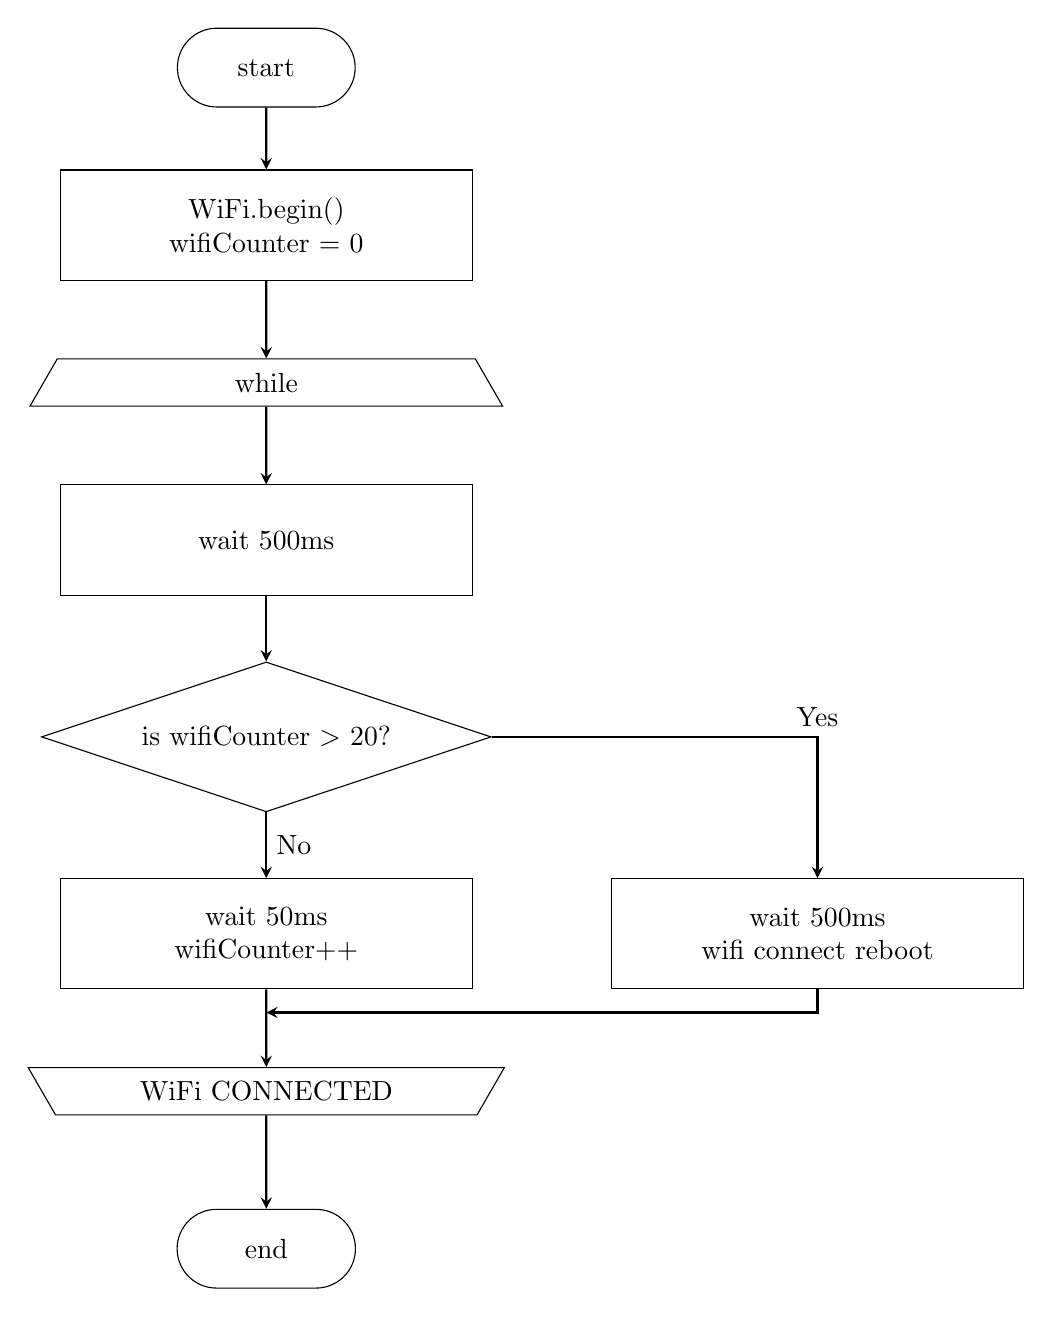
\begin{tikzpicture}
\tikzset{Terminal/.style={rounded rectangle,  draw,  text centered, text width=2cm, minimum height=1cm}};
\tikzset{Process/.style={rectangle,  draw,  text centered, text width=5cm, minimum height=1.4cm}};
\tikzset{ifthen/.style={diamond,  draw,  text centered, aspect=3,text width=4cm, minimum height=1cm}};
\tikzset{InOut/.style={trapezium, draw, text centered, text width=4cm, minimum height=0.6cm, trapezium left angle=70, trapezium right angle=110}};
\tikzset{LoopStart/.style={trapezium, draw, text centered, text width=4cm, minimum height=0.6cm, trapezium angle=60}};
\tikzset{LoopStop/.style={trapezium, draw, text centered, text width=4cm, minimum height=0.6cm, trapezium angle=120}};
\tikzset{arrow/.style={thick, ->, >=stealth}};
\node[Terminal](a)at (0,0){start};
\node[Process](b)at (0,-2){WiFi.begin()\\wifiCounter = 0};
\node[LoopStart](c)at (0,-4){while};
\node[Process](d)at (0,-6){wait 500ms};
\node[ifthen](e)at (0,-8.5){is wifiCounter $>$ 20?};
\node[Process](f)at (0,-11){wait 50ms\\wifiCounter++};
\node[Process](g)at (7,-11){wait 500ms\\wifi connect reboot};
\node[LoopStop](h)at (0,-13){WiFi CONNECTED};
\node[Terminal](i)at (0,-15){end};
\coordinate(j) at (0, -12);

\draw[arrow](a)--(b);
\draw[arrow](b)--(c);
\draw[arrow](c)--(d);
\draw[arrow](d)--(e);
\draw[arrow](e)-- node[anchor=west]{No} (f);
\draw[arrow](e)-| node[anchor=south]{Yes} (g);
\draw[arrow](f)--(h);
\draw[arrow](g)|-(j);
\draw[arrow](h)--(i);
\end{tikzpicture}

\newpage
Arduino (Web request) and IFTTT
\\

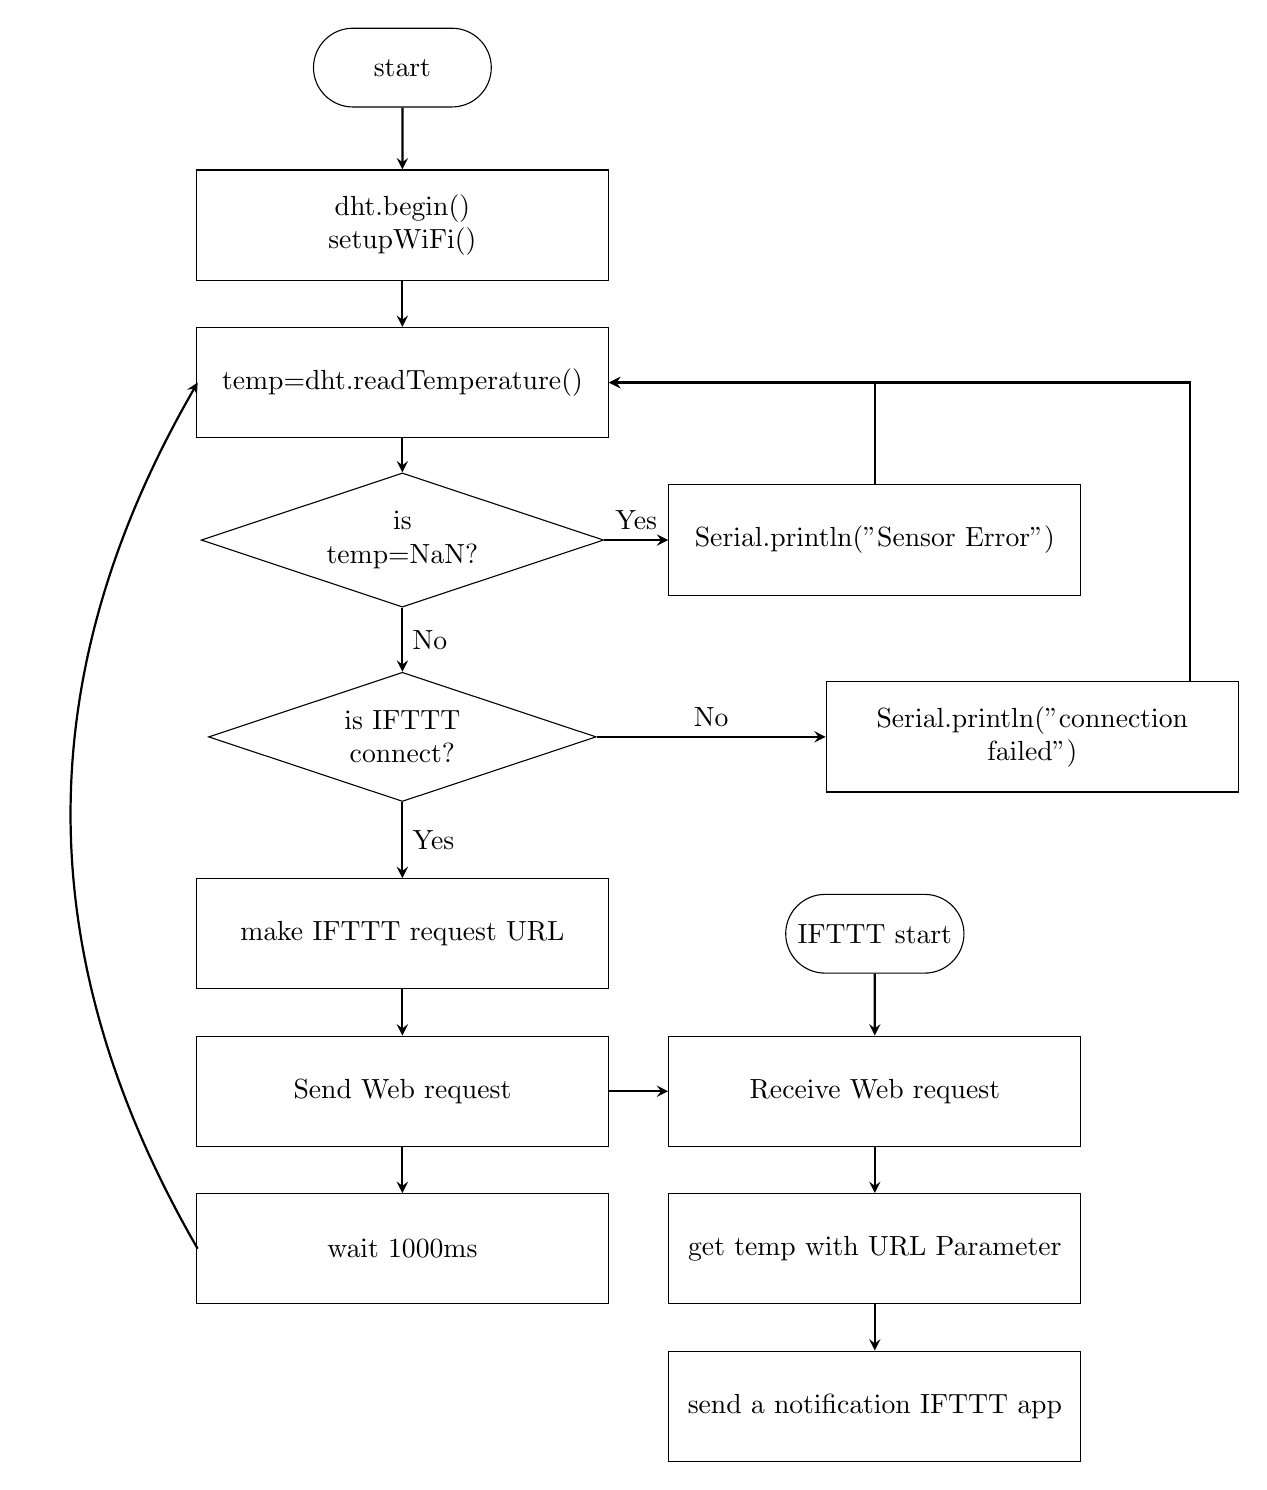
\begin{tikzpicture}
\tikzset{Terminal/.style={rounded rectangle,  draw,  text centered, text width=2cm, minimum height=1cm}};
\tikzset{Process/.style={rectangle,  draw,  text centered, text width=5cm, minimum height=1.4cm}};
\tikzset{ifthen/.style={diamond,  draw,  text centered, aspect=3,text width=2cm, minimum height=1cm}};
\tikzset{InOut/.style={trapezium, draw, text centered, text width=4cm, minimum height=0.6cm, trapezium left angle=70, trapezium right angle=110}};
\tikzset{LoopStart/.style={trapezium, draw, text centered, text width=4cm, minimum height=0.6cm, trapezium angle=60}};
\tikzset{LoopStop/.style={trapezium, draw, text centered, text width=4cm, minimum height=0.6cm, trapezium angle=120}};
\tikzset{arrow/.style={thick, ->, >=stealth}};
\node[Terminal](a)at (0,0){start};
\node[Process](b)at (0,-2){dht.begin()\\setupWiFi()};
\node[Process](c)at (0,-4){temp=dht.readTemperature()};
\coordinate(c1) at (-2.6, -4);
\node[ifthen](d)at (0,-6){is temp=NaN?};
\node[Process](e)at (6,-6){Serial.println("Sensor Error")};
\node[ifthen](f)at (0,-8.5){is IFTTT connect?};
\node[Process](g)at (8,-8.5){Serial.println("connection failed")};
\coordinate(g1) at (10, -7.8);
\node[Process](h)at (0,-11){make IFTTT request URL};
\node[Terminal](i)at (6,-11){IFTTT start};
\node[Process](j)at (0,-13){Send Web request};
\node[Process](k)at (6,-13){Receive Web request};
\node[Process](l)at (0,-15){wait 1000ms};
\coordinate(l1) at (-2.6, -15);
\node[Process](m)at (6,-15){get temp with URL Parameter};
\node[Process](n)at (6,-17){send a notification IFTTT app};

\draw[arrow](a)--(b);
\draw[arrow](b)--(c);
\draw[arrow](c)--(d);
\draw[arrow](d)-- node[anchor=south]{Yes} (e);
\draw[arrow](e)|-(c);
\draw[arrow](d)-- node[anchor=west]{No} (f);
\draw[arrow](f)-- node[anchor=south]{No} (g);
\draw[arrow](g1)|-(c);
\draw[arrow](f)-- node[anchor=west]{Yes} (h);
\draw[arrow](h)--(j);
\draw[arrow](i)--(k);
\draw[arrow](j)--(k);
\draw[arrow](j)--(l);
\draw[arrow](k)--(m);
\draw[arrow](m)--(n);
\draw[arrow](l1)to [bend left](c1);
\end{tikzpicture}

\newpage
\begin{thebibliography}{99}
    \bibitem{ref} Arduino公式リファレンス 日本語訳ページ https://garretlab.web.fc2.com/arduino\_reference/
    \bibitem{DHTgit} GitHub DHT-sensor-library DHTtester.ino https://github.com/adafruit/DHT-sensor-library/blob/master/examples/DHTtester/DHTtester.ino
\end{thebibliography}


\end{document}